\section{Discussion}
\subsection{Fairness Analysis on Tabular Data}
First if we compare the clustered PCA made with the Anchors method and with SHAP method, we can notice that the Anchors one distinguish better a region of gendered anchors.

It's significant to compare the bottom line of each Figure, that shows the filtered explanations based on high predictions and in which the 'SEX' variable in relevant to the explanation, being in the top-3 of the ranking of SHAP values or being in an anchor with a ceiling of 3 features.

So if we compare the distribution of the explanations in an Anchors approach (Figures \ref{fig:clusters_xg_tx_anchors} and \ref{fig:clusters_skrub_tx_anchors}) and SHAP approach (Figures \ref{fig:clusters_xg_tx_shap} and \ref{fig:clusters_skrub_tx_shap}), we can have more relevant insights in the Anchors one. That can be due the fact that the anchor generated by the method tests the features that are crucial to keep the prediction always the same in a local explanation, different than SHAP that gives a weight and rank the features in importance, to any feature that affects the prediction in a positive way.

For further analysis we will set the labels to reference the clusters as:
\begin{itemize}
    \item Cluster 1 - the cluster located in the bottom left of the plots
    \item Cluster 2 - the cluster located in the top of the plots
    \item Cluster 3 - the cluster located in the bottom right of the plots
\end{itemize}

Focusing on the Anchors method we can notice a concentration of gendered anchors on Clusters 1 and 2, it's important to try to understand what are the profiles of the people in each cluster, so we took the PC1 and PC2 to analyse what are the features with higher weights on each component.

\begin{table}[h]
\centering
\caption{Folktables Dataset Features}
\label{tab:folktables-pca-profiles}
\begin{tabular}{lrr}
\hline
\textbf{Feature code} & \textbf{PCA 1 (axis X)}  & \textbf{PCA 2 (axis Y)} \\
\hline
AGEP & \textbf{-0.48} & 0.24 \\
COW & -0.24 & 0.01 \\
SCHL & -0.29 & \textbf{-0.49} \\
MAR & \textbf{0.52} & -0.29 \\
OCCP & \textbf{0.31} & \textbf{0.39} \\
POBP & 0.10 & \textbf{0.51} \\
RELP & \textbf{0.45} & -0.15 \\
WKHP & -0.17 & 0.17 \\
SEX & -0.03 & \textbf{-0.30} \\
RAC1P & 0.15 & 0.26 \\
\hline
\end{tabular}
\end{table}

In the Table \ref{tab:folktables-pca-profiles} we can take the four higher values to analyse the profiles of each axis.

\begin{enumerate}
    \item PC 1 - Axis X
    \begin{enumerate}
        \item MAR (positive)
        \begin{enumerate}
            \item $\uparrow$ PC 1: means less probability of being married (MAR $> 1 \Rightarrow $ widowed, divorced, separated, never married or under 15 years old)
            \item $\downarrow$ PC 1: means more probability of being married (MAR $= 1 \Rightarrow $ married)
        \end{enumerate}

        \item AGEP (negative)
        \begin{enumerate}
            \item $\uparrow$ PC 1: means more probability of being younger
            \item $\downarrow$ PC 1: means more probability of being older
        \end{enumerate}

        \item RELP (positive)
        \begin{enumerate}
            \item $\uparrow$ PC 1: means more probability of being in a traditional family relationship at the house
            \item $\downarrow$ PC 1: means more probability of being in a different or non-traditional relashionship at the house
        \end{enumerate}

        \item OCCP (positive)
        \begin{enumerate}
            \item $\uparrow$ PC 1: means more probability of being in a high-skill, high-status occupation often requiring advanced education (e.g., management, engineering, law, medicine).
            \item $\downarrow$ PC 1: means more probability of being in a  lower-skill, manual, or service-oriented occupation that often requires less formal education or is based on on-the-job training (e.g., construction, transportation, cleaning, farming). 
        \end{enumerate}
    \end{enumerate}

    \item PC 2 - Axis Y
    \begin{enumerate}
        \item POBP (positive)
        \begin{enumerate}
            \item $\uparrow$ PC 2: means more probability of being an immigrant (higher codes are associated to people born outside of the USA)
            \item $\downarrow$ PC 2: means more probability of being a person born in the USA
        \end{enumerate}

        \item SCHL (negative)
        \begin{enumerate}
            \item $\uparrow$ PC 2: means more probability of being a person with a low level of education
            \item $\downarrow$ PC 2: means more probability of being a person with a high level of education
        \end{enumerate}

        \item OCCP (positive)
        \begin{enumerate}
            \item $\uparrow$ PC 2: means more probability of being in a high-skill, high-status occupation often requiring advanced education (e.g., management, engineering, law, medicine).
            \item $\downarrow$ PC 2: means more probability of being in a  lower-skill, manual, or service-oriented occupation that often requires less formal education or is based on on-the-job training (e.g., construction, transportation, cleaning, farming). 
        \end{enumerate}

        \item SEX (negative)
        \begin{enumerate}
            \item $\uparrow$ PC 2: means more probability of being a man (SEX $= 1 \Rightarrow $ male)
            \item $\downarrow$ PC 2: means more probability of being a woman (SEX $= 2 \Rightarrow $ female)
        \end{enumerate}
    \end{enumerate}
\end{enumerate}

Combining the clusters with the PCA analysis, we can build a profile for each cluster:

\begin{itemize}
    \item \textbf{Cluster 1: Established, Working-Class, US-born Women.} This cluster consists of older, married women born in the US, likely settled into traditional family structures and working in occupations that require less or medium formal education.
    
    \item \textbf{Cluster 2: Young, Immigrant, and Professionally Diverse Men.} This is the most diverse cluster, encompassing younger immigrant men who are not married. It includes both high-skill professionals and lower-skill laborers, representing the broad spectrum of the immigrant experience.

    \item \textbf{Cluster 3: Young, US-born, Entry-Level Service Workers.} This cluster consists of the youngest adults, born in the US, who are not married and are just starting out in the workforce, typically in low-wage, low-skill jobs with high economic vulnerability.
\end{itemize}

Seeing the generated profiles we can relate to the gendered anchors points. These points will be heavily concentrated in the bottom right-half of the plot (low PC2, which is associated with being female) and likely spread across Cluster 1 (bottom left), a part of Cluster 2 and a small female portion of Cluster 3 (bottom right).

This pattern is so common it applies to over 10\% of the population in the test set, as the coverage metric shows. That concentration can show mainly a bias between older married women and still a strong bias between immigrant women.

This type of result can lead us to think of public policies to help this population and remediate the unfairness in these specific populations.

For further proving that the Anchors really mark an area of bias we also did some tests to calculate the Disparate Impact in the area with the gendered anchors. We will use for this test the plot on the Figure \ref{fig:clusters_skrub_tx_anchors} that used the HistGradientBoosting for generating the Anchors, and that has the lowest DI between it and XGBoost.
So we selected the square around the concentrated area as shown in Figure \ref{fig:square_cluster} with coordinates $PC1 = [-2, 0]$ and $PC2 = [-2, 0]$ to calculate the DI and verify that the value is lower or similar to the DI of the whole state. In this region we have 4011 individuals, being 1300 men and 2711 women, and a DI of 0.46 with an interval of confidence of [0.44, 0.48].

\begin{figure}[h]
    \centering
    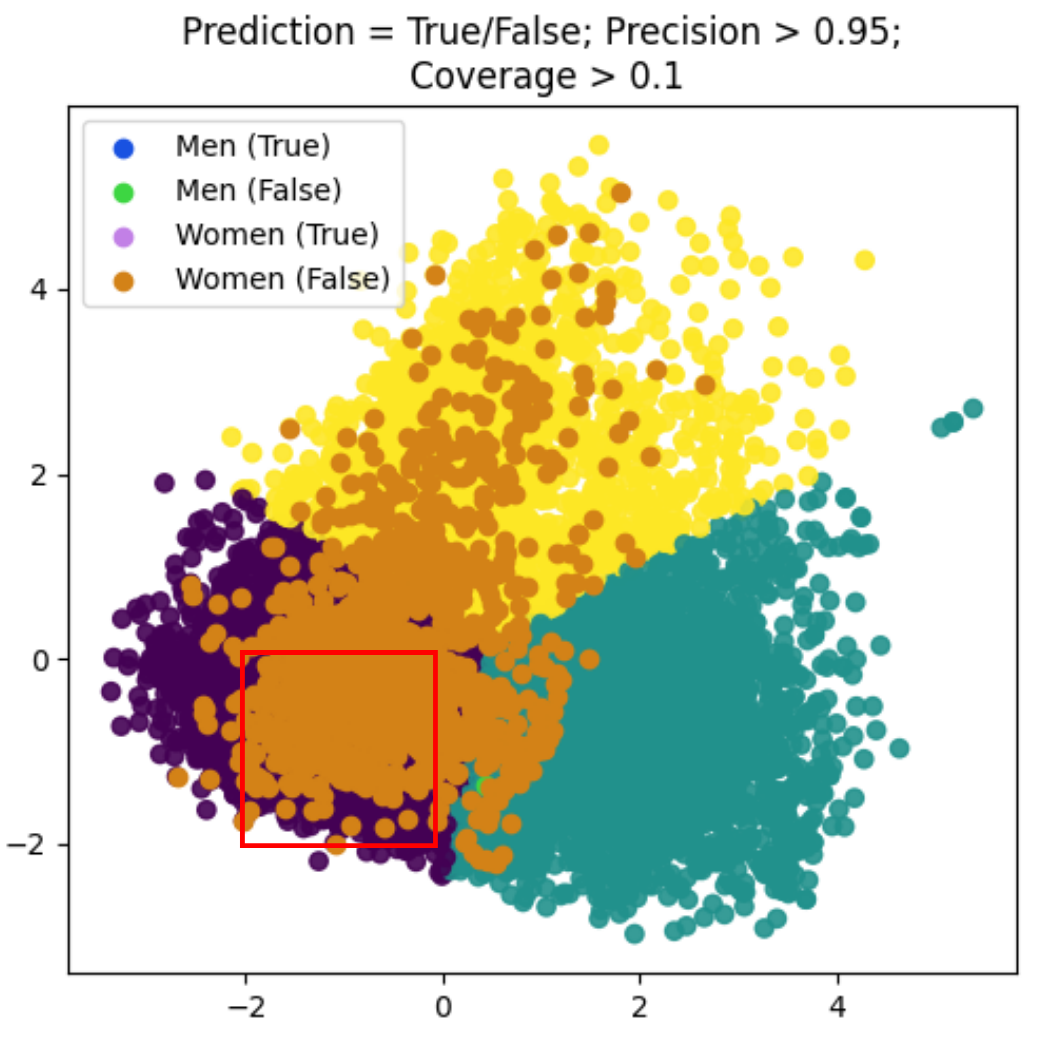
\includegraphics[width=0.7\textwidth]{Images/clustered_pca_square.png}
    \caption{Selected group of the clustered PCA in the Texas state, Model: HistGradientBoosting and XAI method: Anchors. Red square with coordinates $PC1 = [-2, 0]$ and $PC2 = [-2, 0]$}
    \label{fig:square_cluster}
\end{figure}

The DI of Texas is already very low (0.54) (Figure \ref{tab:folktables-results}), but in the region showed it can be even lower (0.46), proving that the Anchors is highligtning a region with high unfairness.

\FloatBarrier

\subsection{"Anchors Regression" applied on Multi-dimensional Data}
Having implemented our Regression Anchors approach on a simplified model with three channels, we subsequently conducted tests on other model configurations to evaluate its robustness and scalability. The configurations are described as follows:

\begin{enumerate}
\item \textbf{Rain Model (No Boundaries):} Trained exclusively on the three AROME rain channels (channels 7, 8, and 13 in Table \ref{tab:meteo_channels}), as presented in the previous results.
\item \textbf{Rain Model (With Boundaries):} Trained on the three AROME rain channels (7, 8, 13) augmented with all ARPÈGE global fields (channels 22--37) as boundary conditions.
\item \textbf{Full Model (No Boundaries):} Trained on the complete set of 21 AROME channels (1--21), without boundary conditions.
\item \textbf{Full Model (With Boundaries):} Trained on the full suite of AROME channels (1--21) combined with all ARPÈGE global fields (22--37) to provide boundary conditions.
\end{enumerate}

The following configurations were used for generating the anchors across all models:
\begin{itemize}
    \item Sampling period: November 2023.
    \item Number of counterfactuals:
    \begin{itemize}
        \item $K = 300$ for the Rain Model (lower dimensionality).
        \item $K = 2,000$ for the Full Model (higher dimensionality).
    \end{itemize}
    \item Center of target location: Centered on $(i, j)$.
    \begin{itemize}
        \item Spatial extent of the center of the perturbation mask: $\sigma_d = 150$ pixels.
    \end{itemize}
    \item Center of perturbation mask: Centered on $(\widehat{i_k}, \widehat{j_k})$.
    \begin{itemize}
        \item Spatial extent of the perturbation mask: $\sigma_e = 20$ pixels.
    \end{itemize}
    \item Prediction difference threshold: $\epsilon = 0.05$ (i.e., the prediction is considered to have changed if it varies by more than 5\%).
\end{itemize}

Focusing on a particularly illustrative case, we conducted tests on data from November $21^{st}$ for the target location $(i, j) = (300, 250)$ (near Limoges).

The results for the different models are presented in the following figures:
\begin{itemize}
\item Figure \ref{fig:titan-rain-anchors-21}: Rain Model (No Boundaries)
\item Figure \ref{fig:titan-rain-arp-anchors-21}: Rain Model (With Boundaries)
\item Figure \ref{fig:titan-full-anchors-21}: Full Model (No Boundaries)
\item Figure \ref{fig:titan-full-arp-anchors-21}: Full Model (With Boundaries)
\end{itemize}

It is important to note that the Rain Model with Boundaries did not yield satisfactory results. This is likely due to a data discrepancy: while the Rain Model is trained on lower-atmosphere AROME channels, the ARPÈGE inputs only provide atmospheric data from 250 hPa upwards. This mismatch in vertical resolution probably hindered the model's ability to integrate the boundary conditions effectively. Consequently, the following discussion will focus on the results from the Rain Model without Boundaries.

For the Full Model results, we display only the channels that contained anchors, not all 21 channels. The results for the Full Model without Boundaries can be interpreted by considering two factors: the number of anchors per channel (indicating influence) and the magnitude of their effect on the prediction.

Comparing the results of the Full Model with and without boundaries reveals that the model trained with ARPÈGE data produced more conservative explanations. It generated anchors in fewer channels and with a lower density per channel. This increased selectivity may be due to the robustness introduced by the global context provided by the ARPÈGE boundary conditions. Despite this difference, there is an intersection between the anchors found in both models (Figures \ref{fig:titan-full-arp-anchors-21} and \ref{fig:titan-full-anchors-21}), indicating agreement on the importance of certain channels and locations.

\begin{figure}[h]
    \centering
    \begin{subfigure}[b]{0.49\textwidth}
        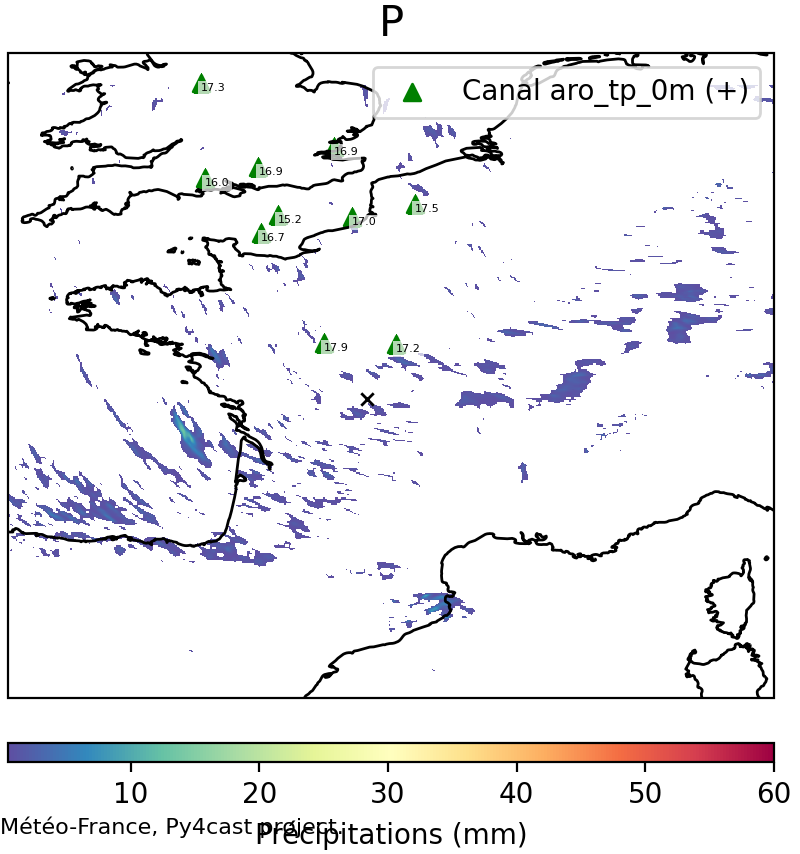
\includegraphics[width=\textwidth]{Images/titan_rain_anchors/nov-21/rain-arp/2023112100_feature_aro_tp_0m.png}
        \caption{Channel aro\_tp\_0m}
    \end{subfigure}
    \hfill
    \begin{subfigure}[b]{0.49\textwidth}
        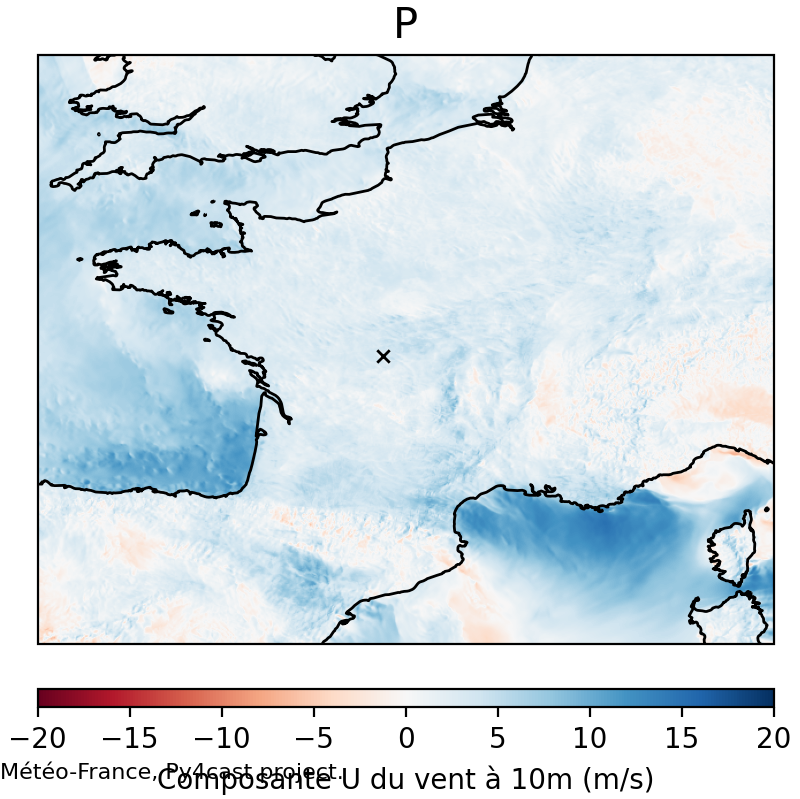
\includegraphics[width=\textwidth]{Images/titan_rain_anchors/nov-21/rain-arp/2023112100_feature_aro_u10_10m.png}
        \caption{Channel aro\_u10\_10m}
    \end{subfigure}
    \hfill
    \begin{subfigure}[b]{0.49\textwidth}
        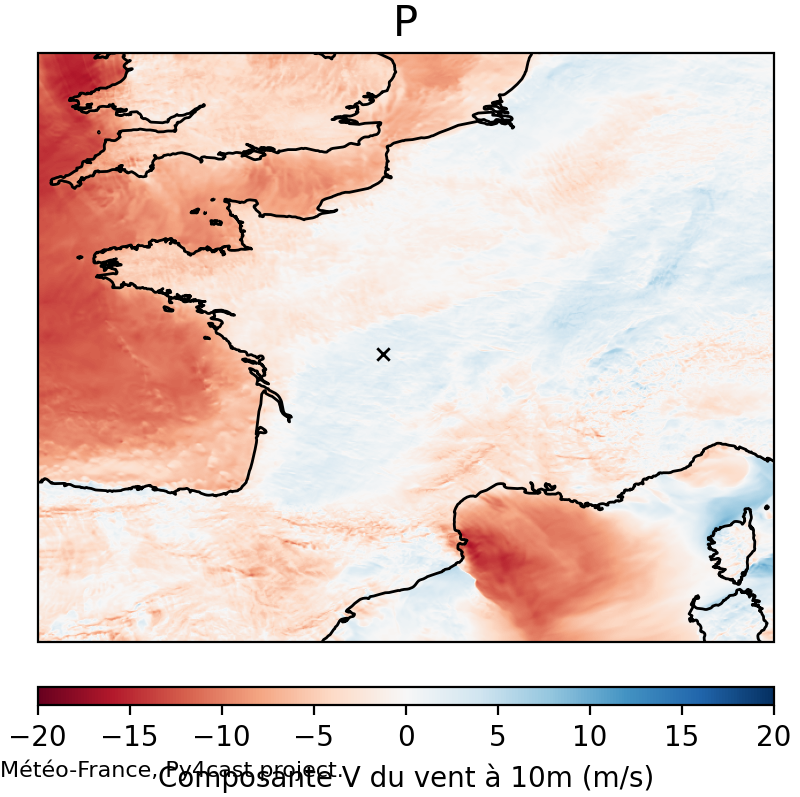
\includegraphics[width=\textwidth]{Images/titan_rain_anchors/nov-21/rain-arp/2023112100_feature_aro_v10_10m.png}
        \caption{Channel aro\_v10\_10m}
    \end{subfigure}
    \caption{Example of anchors applied on Rain Model (With Boundaries), on $21^{st}$ November data.}
    \label{fig:titan-rain-arp-anchors-21}
\end{figure}

\begin{figure}[h]
    \centering
    \begin{subfigure}[b]{0.44\textwidth}
        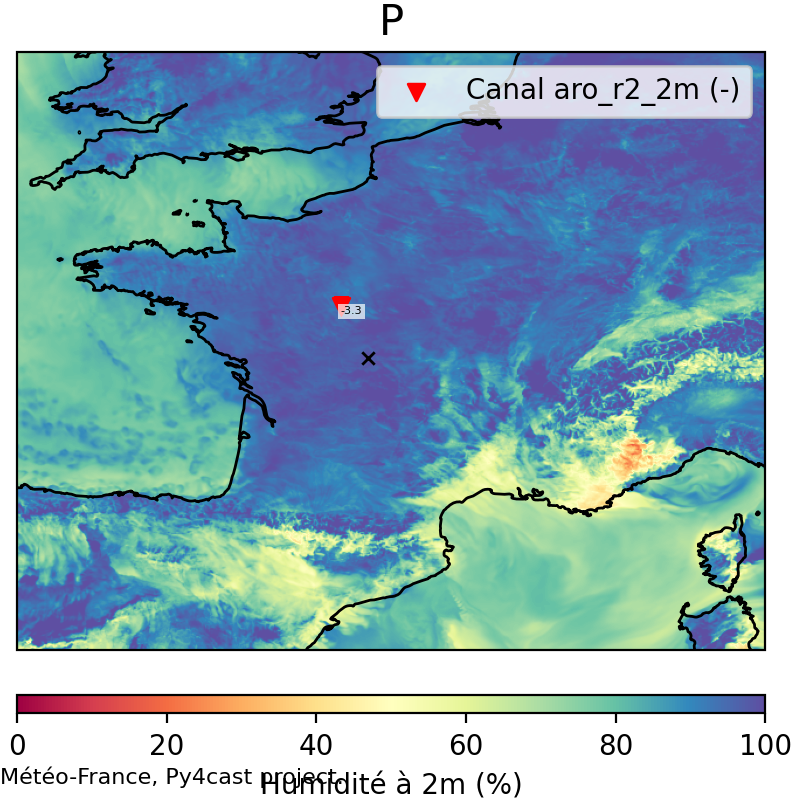
\includegraphics[width=\textwidth]{Images/titan_rain_anchors/nov-21/complete/2023112100_feature_aro_r2_2m.png}
        \caption{Channel aro\_r2\_2m}
    \end{subfigure}
    \hfill
    \begin{subfigure}[b]{0.44\textwidth}
        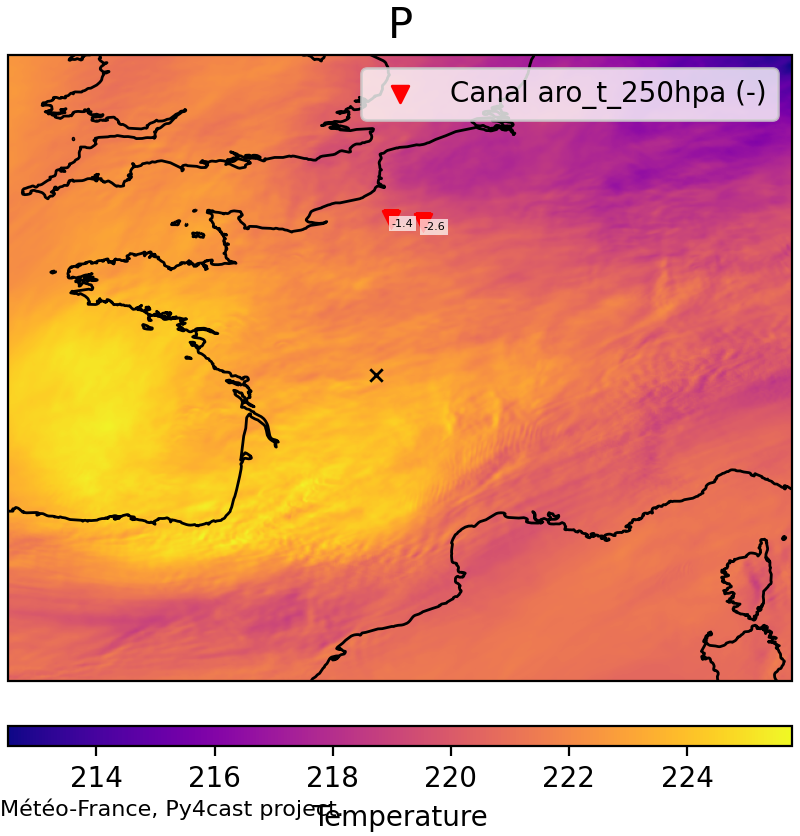
\includegraphics[width=\textwidth]{Images/titan_rain_anchors/nov-21/complete/2023112100_feature_aro_t_250hpa.png}
        \caption{Channel aro\_t\_250hpa}
    \end{subfigure}
    \hfill
    \begin{subfigure}[b]{0.44\textwidth}
        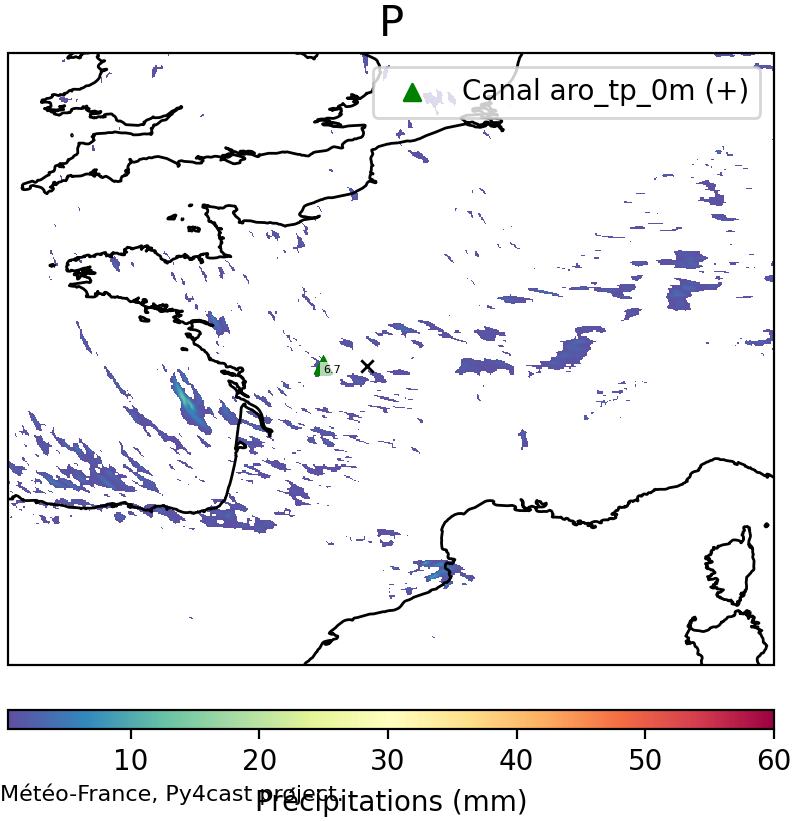
\includegraphics[width=\textwidth]{Images/titan_rain_anchors/nov-21/complete/2023112100_feature_aro_tp_0m.png}
        \caption{Channel aro\_tp\_0m}
    \end{subfigure}
    \hfill
    \begin{subfigure}[b]{0.44\textwidth}
        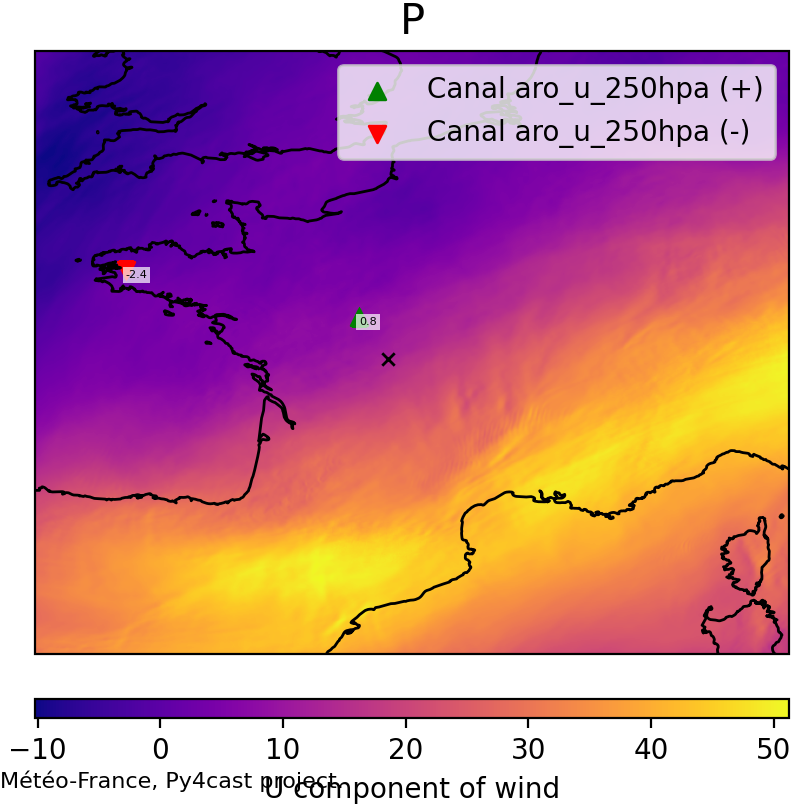
\includegraphics[width=\textwidth]{Images/titan_rain_anchors/nov-21/complete/2023112100_feature_aro_u_250hpa.png}
        \caption{Channel aro\_u\_250hpa}
    \end{subfigure}
    \hfill
    \begin{subfigure}[b]{0.44\textwidth}
        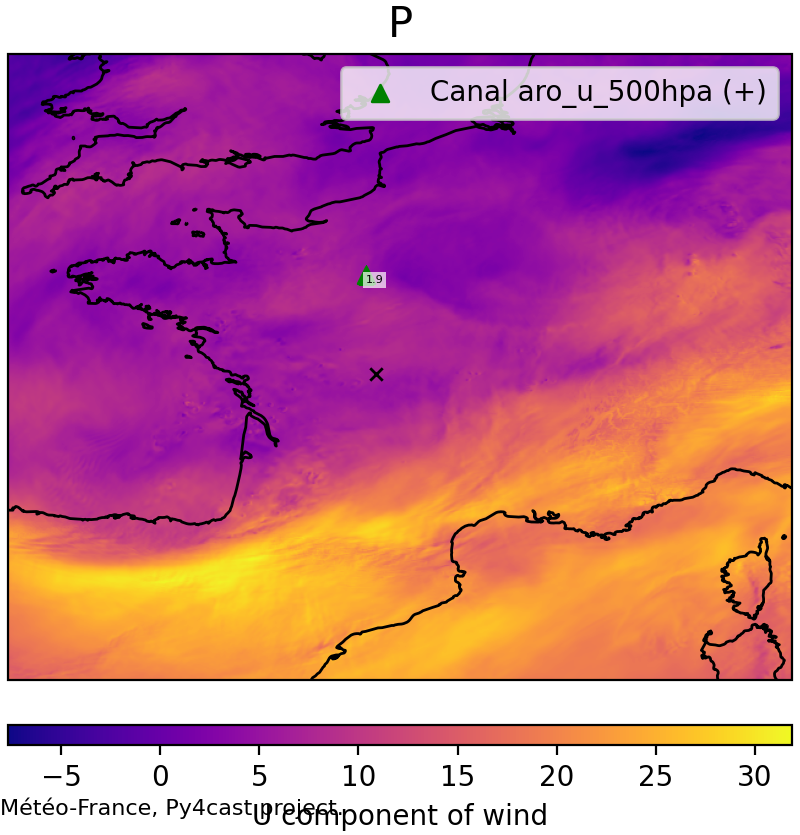
\includegraphics[width=\textwidth]{Images/titan_rain_anchors/nov-21/complete/2023112100_feature_aro_u_500hpa.png}
        \caption{Channel aro\_u\_500hpa}
    \end{subfigure}
    \hfill
    \begin{subfigure}[b]{0.44\textwidth}
        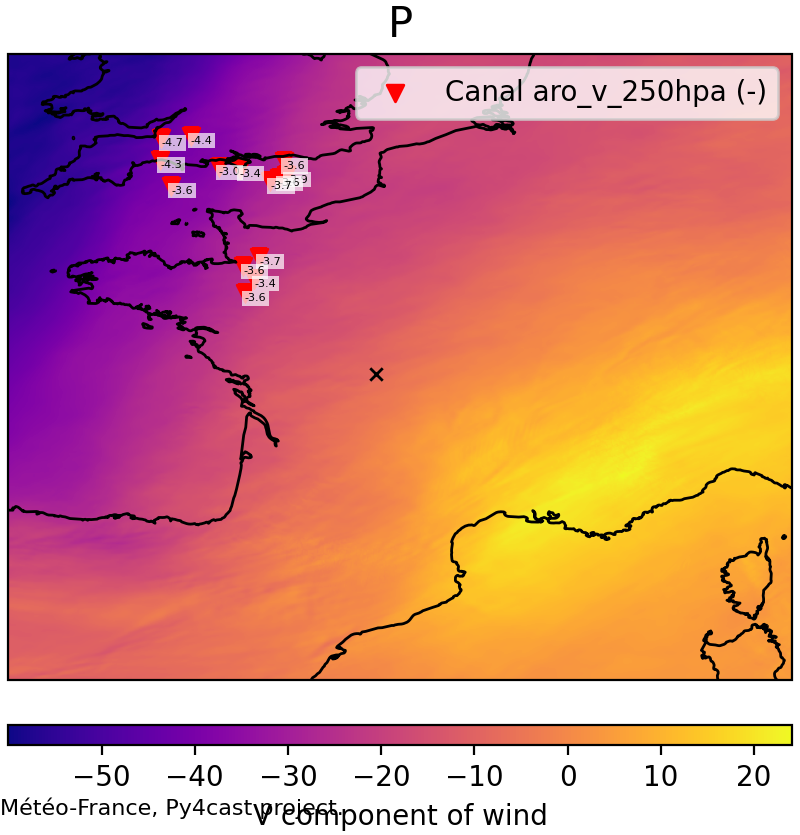
\includegraphics[width=\textwidth]{Images/titan_rain_anchors/nov-21/complete/2023112100_feature_aro_v_250hpa.png}
        \caption{Channel aro\_v\_250hpa}
    \end{subfigure}
    \caption{Anchors applied on Full Model (No Boundaries), on $21^{st}$ November data. (Part 1)}
\end{figure}

\begin{figure}[h]
    \ContinuedFloat
    \begin{subfigure}[b]{0.44\textwidth}
        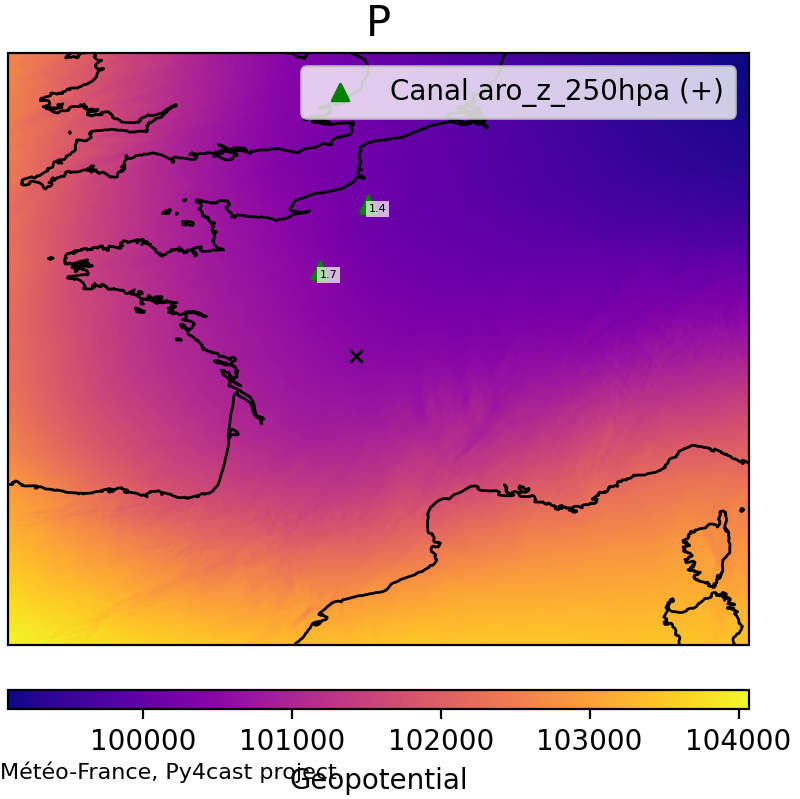
\includegraphics[width=\textwidth]{Images/titan_rain_anchors/nov-21/complete/2023112100_feature_aro_z_250hpa.png}
        \caption{Channel aro\_z\_250hpa}
    \end{subfigure}
    \hfill
    \begin{subfigure}[b]{0.44\textwidth}
        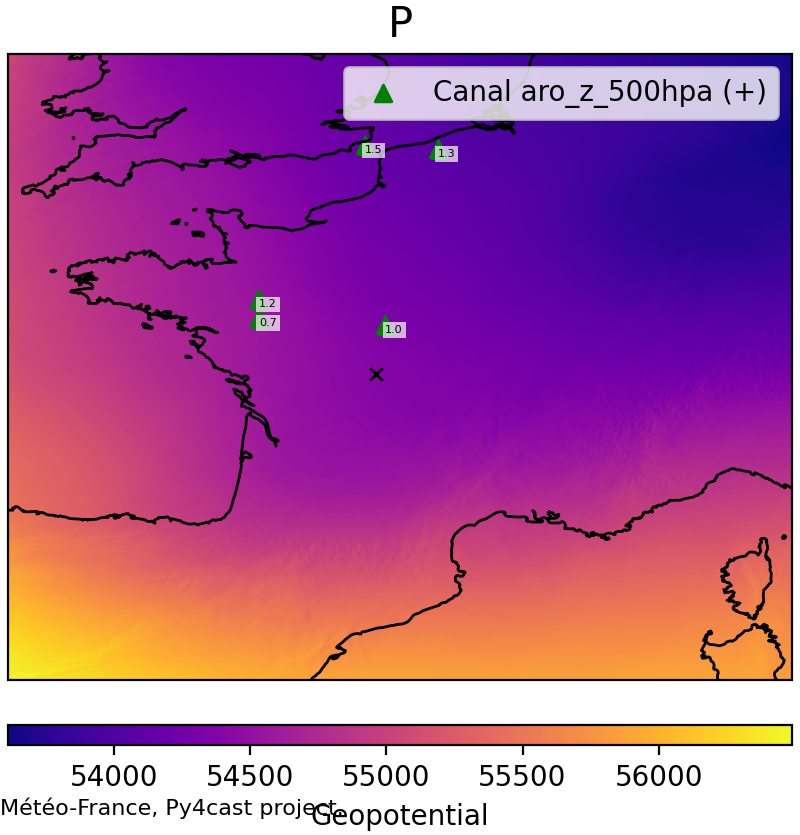
\includegraphics[width=\textwidth]{Images/titan_rain_anchors/nov-21/complete/2023112100_feature_aro_z_500hpa.png}
        \caption{Channel aro\_z\_500hpa}
    \end{subfigure}
    \hfill
    \begin{subfigure}[b]{0.44\textwidth}
        \includegraphics[width=\textwidth]{Images/titan_rain_anchors/nov-21/complete/2023112100_feature_aro_z_700hpa.png}
        \caption{Channel aro\_z\_700hpa}
    \end{subfigure}
    \hfill
    \begin{subfigure}[b]{0.44\textwidth}
        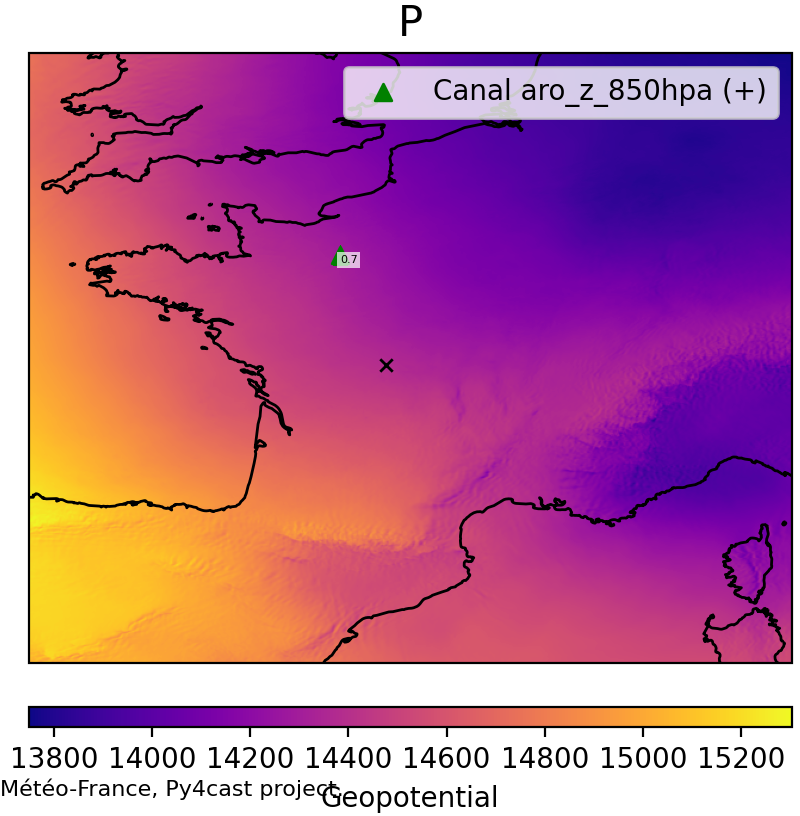
\includegraphics[width=\textwidth]{Images/titan_rain_anchors/nov-21/complete/2023112100_feature_aro_z_850hpa.png}
        \caption{Channel aro\_z\_850hpa}
    \end{subfigure}
    \caption{Anchors applied on Full Model (No Boundaries), on $21^{st}$ November data. (Part 2)}
    \label{fig:titan-full-anchors-21}
\end{figure}

  
\begin{figure}[h]
    \centering
    \begin{subfigure}[b]{0.49\textwidth}
        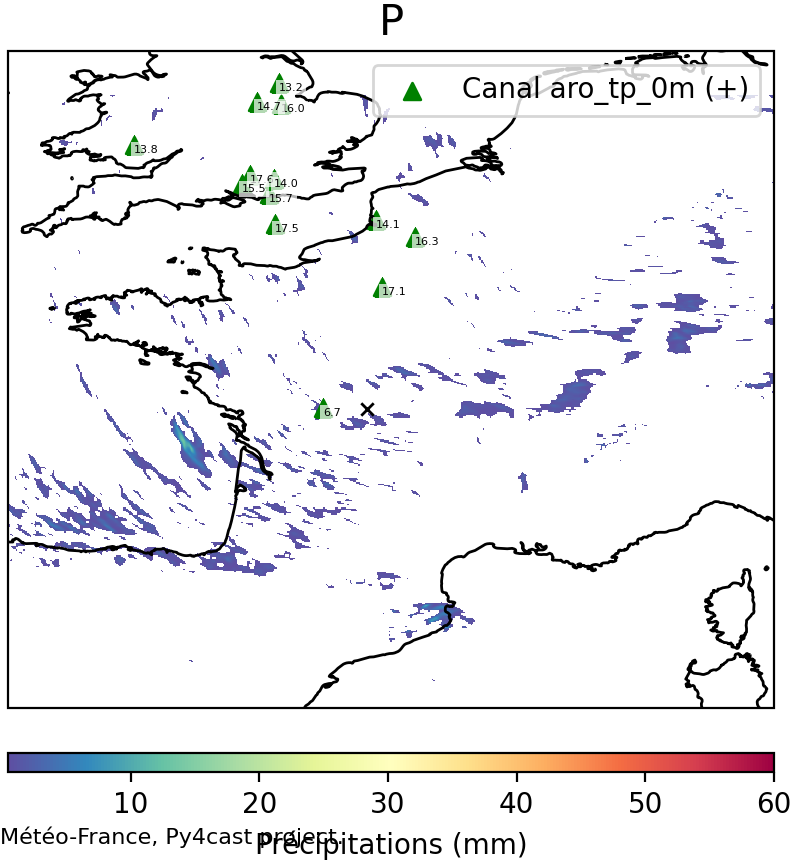
\includegraphics[width=\textwidth]{Images/titan_rain_anchors/nov-21/complete-arp/2023112100_feature_aro_tp_0m.png}
        \caption{Channel aro\_tp\_0m}
    \end{subfigure}
    \hfill
    \begin{subfigure}[b]{0.49\textwidth}
        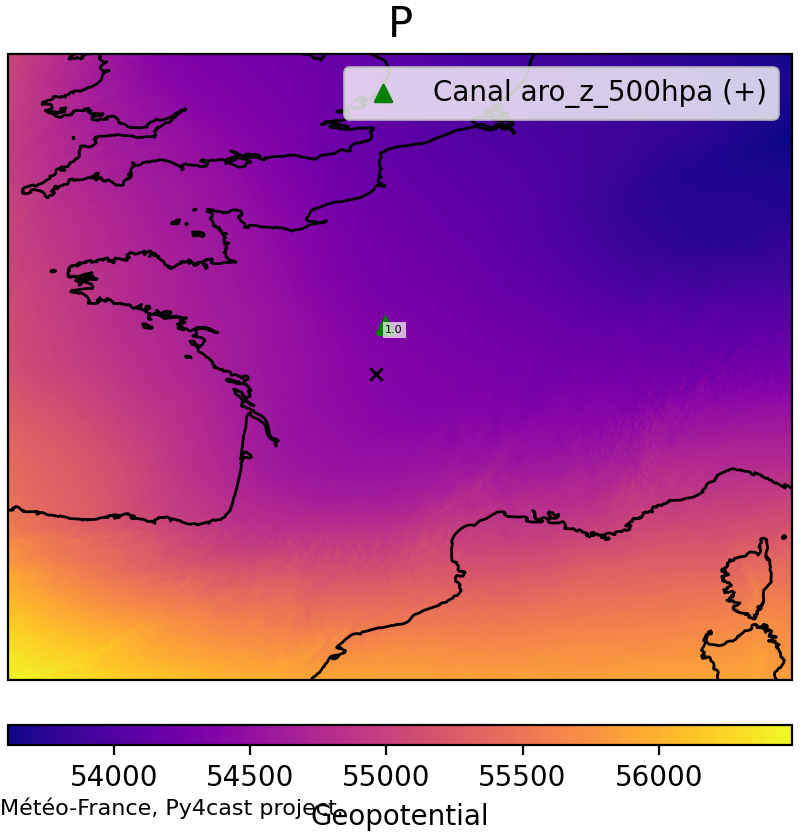
\includegraphics[width=\textwidth]{Images/titan_rain_anchors/nov-21/complete-arp/2023112100_feature_aro_z_500hpa.png}
        \caption{Channel aro\_z\_500hpa}
    \end{subfigure}
    \hfill
    \begin{subfigure}[b]{0.49\textwidth}
        \includegraphics[width=\textwidth]{Images/titan_rain_anchors/nov-21/complete-arp/2023112100_feature_aro_z_700hpa.png}
        \caption{Channel aro\_z\_700hpa}
    \end{subfigure}
    \caption{Anchors applied on Full Model (With Boundaries), on $21^{st}$ November data. (Part 1)}
    \label{fig:titan-full-arp-anchors-21}
\end{figure}

\subsection{"Anchors Regression" applied on LLM}
The application of the "Regression Anchors" method to high-dimensional, spatial-temporal data, as demonstrated in weather forecasting, establishes a versatile framework that can be adapted to other complex domains. A direct and promising extension would be to LLMs.

The core methodology remains applicable: one would define a precise prediction to explain (e.g., a model's sentiment score or its choice of a specific token) and generate counterfactuals by perturbing the input. The concept of a spatial perturbation mask would be translated into a textual mask, where certain words or tokens in a sentence are perturbed or replaced according to a defined strategy. The precision and coverage metrics would then identify the minimal set of words (the "anchor") that most reliably controls the model's output.

While the exciting prospect of applying this methodology to LLMs was beyond the scope of this internship due to time constraints, it represents a logical and valuable progression for this research, bridging explainability between perceptual (vision/weather) and semantic (language) AI systems.